\section{The \tlaplus\ Proof Language}

\begin{frame}
  \frametitle{Assertions}

  \begin{itemize}
  \item \tc{dkblue}{Assertions state valid facts}

  \oo \tc{dkblue}{\AXIOM\ and \ASSUME\ assert unproved facts}

    \begin{itemize}
    \o \tlaps\ handles \ASSUME\ and \AXIOM\ identically
    \o \tlc\ checks \ASSUME{}d facts
    \end{itemize}

  \oo \tc{dkblue}{\THEOREM\ asserts that a fact is provable in the current context}

    \begin{itemize}
    \o the proof need not be given at once
    \o unproved theorems will be colored yellow in the toolbox
    \o \LEMMA\ and \PROPOSITION\ are synonyms of \THEOREM
    \end{itemize}

  \oo \tc{dkblue}{Facts can be named for future reference}

    \medskip

    \begin{tlablock}[.89]
      \THEOREM\ Fermat\ \deq\ \forall n \in Nat \setminus (0..2): \forall a,b,c \in Nat \setminus \{0\}: a^n + b^n \neq c^n
    \end{tlablock}

  \end{itemize}
\end{frame}

\begin{frame}
  \frametitle{Shape of Assertions}

  \begin{itemize}
  \item \tc{dkblue}{A \tlaplus\ assertion can be a formula or a logical sequent}

    \medskip

    \qquad\begin{tlablock}[.7]
      \qquad $F$
      \qquad\qquad\text{or}\qquad\qquad
      \begin{array}{@{}l@{\ \ }l}
        \ASSUME & A_1, \ldots, A_n\\
        \PROVE  & F
      \end{array}
    \end{tlablock}

  \oo \tc{dkblue}{Shape of a sequent \ASSUME\ \ldots\ \PROVE}

    \begin{itemize}
    \o the conclusion $F$ is always a formula

    \o the assumptions $A_i$ can be 

      \medskip

      \begin{tabular}{ll}
        declarations & \tc{dkgreen}{$\NEW\ msg \in Msgs$}\\
                     & (levels: \CONSTANT, \STATE, \ACTION, \TEMPORAL)\\[2mm]
        formulas & \tc{dkgreen}{$msg.type = \str{alert}$}\\[2mm]
        sequents & 
        \tc{dkgreen}{\(\begin{array}[t]{@{}l@{\ \ }l}
          \ASSUME & \NEW\ msg \in Msgs,\ msg.type = \str{alert}\\
          \PROVE  & msg \in Alarm
        \end{array}\)}
      \end{tabular}
    \end{itemize}
  \end{itemize}
\end{frame}

\begin{frame}
  \frametitle{Nested \ASSUME\ \ldots\ \PROVE}

  \begin{itemize}
  \item \tc{dkblue}{Useful for writing proof rules}

    \bigskip

    \begin{tlablock}
      \THEOREM\ ForallIntro\ \deq
      \begin{array}[t]{l@{\ \ }l}
        \ASSUME & \NEW\ P(\_),\\
                & \ASSUME\ \ \NEW\ y\ \ \PROVE\ \ P(y)\\
        \PROVE  & \A x : P(x)
      \end{array}
    \end{tlablock}

    \bigskip

  \item \tc{dkblue}{Nested \ASSUME\ \ldots\ \PROVE\ encodes freshness of $y$}
  \end{itemize}
\end{frame}

\begin{frame}
  \frametitle{Proof Rules in \tlaplus}

  \centerline{\begin{tlablock}
    \THEOREM\ RuleINV1\ \deq\ 
    \begin{array}[t]{@{}l@{\ \ }l}
      \ASSUME & \STATE\ I,\ \STATE\ v,\ \ACTION\ N,\\
              & I \land [N]_v \implies I'\\
      \PROVE  & I \land \Box[N]_v \implies \Box I
    \end{array}
  \end{tlablock}}

  \begin{itemize}
  \oo \tc{dkblue}{Validity of conclusion follows from validity of hypotheses}

    \begin{itemize}
    \o given a substitution of the declared identifiers 

      by expressions of the declared or lower level

    \o if all hypotheses are provable in the current context

       then the instance of the conclusion may be concluded 
    \end{itemize}

\pause

  \oo \tc{dkblue}{Constant-level rules may be instantiated at any level}

    \smallskip

    \centerline{\begin{tlablock}
      \THEOREM\ Substitutivity\ \deq\ 
      \begin{array}[t]{@{}l@{\ \ }l}
        \ASSUME & \NEW\ x,\ \NEW\ y,\ \NEW\ P(\_),\\
                & x=y\\
        \PROVE  & P(x) \biimplies P(y)
      \end{array}
    \end{tlablock}}

    \begin{itemize}
    \o expression instantiating $P(\_)$ must satisfy Leibniz condition
    \end{itemize}
  \end{itemize}
\end{frame}

\begin{frame}
  \frametitle{Structure of \tlaplus\ Proofs}

  \begin{itemize}
  \item \tc{dkblue}{Proofs are either leaf proofs \ldots}

    \smallskip

    \qquad\begin{tlablock}
      \LEMMA\ \ Init \implies InductiveInvariant\\
      \BY\ Positive\ \DEFS\ Init, InductiveInvariant
    \end{tlablock}

\pause

  \oo \tc{dkblue}{\ldots\ or sequences of assertions followed by \QED}

    \smallskip

    \qquad\begin{tlablock}
      \begin{array}{@{}l@{\ \ }l@{\ }l}
        \ps{1}{a.} & \CASE & x<y\\
        \ps{1}{b.} & \CASE & x>y\\
        \ps{1}{q.} & \QED  & \BY\ \ps{1}{a}, \ps{1}{b}
      \end{array}
    \end{tlablock}

    \begin{itemize}
    \o \makebox[8.5cm][l]{every step of a proof has the same \alert{level number}}
       \tc{dkgreen}{$\ps{1}{}$}
    \o \makebox[8.5cm][l]{and may be named for future reference}
       $\ps{1}{\tc{dkgreen}{a.}}$
    \o \QED\ step: the assertion follows from the preceding facts
    \o each step recursively has a proof\ \ $\leadsto$\ \ proof tree
    \o proof step with higher level number starts subproof
    \end{itemize}

  \oo \tc{dkblue}{Proofs are best developed per level (check only \QED\ step)}
  \end{itemize}
\end{frame}

\begin{frame}
  \frametitle{Leaf Proofs}

  \begin{itemize}
  \item \tc{dkblue}{Elementary steps: assertion follows by ``simple reasoning''}

    \medskip

    \begin{tlablock}
      \BY\ e_1, \ldots, e_m\ \DEFS\ d_1, \ldots, d_n
    \end{tlablock}

    \begin{itemize}
    \o \tc{dkgreen}{$e_1, \ldots, e_m$} : known facts (assumptions, theorems, previous steps)
    \o formulas implied by known facts may also appear among $e_i$
    \o \tc{dkgreen}{$d_1, \ldots, d_n$} : operator names whose definitions should be expanded
    \o citation of facts and definitions limits size of proof obligations
    \o \tc{dkgreen}{\OBVIOUS} : assertion follows without use of extra facts
    \end{itemize}

\pause

  \oo \tc{dkblue}{Checking leaf proofs in \tlaps}

    \begin{itemize}
    \o verify that $e_1, \ldots, e_m$ are provable in current context
    \o expand the definitions of $d_1, \ldots, d_n$
    \o pass obligation to a prover (default: Zenon, then Isabelle)
    \o some ``facts'' specify a prover backend, e.g. $SimpleArithmetic$
    \end{itemize}

  \oo \alert{\tlaps\ is independent of axiomatic systems and theorem provers}
  \end{itemize}
\end{frame}

\begin{frame}
  \frametitle{Known and Usable Facts and Definitions}

  \begin{itemize}
  \item \tc{dkblue}{Scoping and context}

    \begin{itemize}
    \o obvious scope rules determine current context
    \o context contains known declarations, facts, and definitions
    \o assertions state that a fact is provable in the current context
    \end{itemize}

  \oo \tc{dkblue}{Usable facts and definitions}

    \begin{itemize}
    \o \alert{usable facts/definitions} : passed to backend provers
    \o facts and definitions must normally be cited explicitly in \BY
    \o \tc{dkgreen}{$\USE\ e_1,\ldots,e_m\ \DEFS\ d_1,\ldots,d_n$}\ \ makes
       facts usable within scope
    \o domain facts\ \ \tc{dkgreen}{$x \in S$}\ \ are usable by default
    \o facts stated in unnamed steps are usable by default
    \o definitions introduced within a proof are usable by default
    \o definitions of theorem names are usable by default
    \o \tc{dkgreen}{$\HIDE\ e_1,\ldots,e_m\ \DEFS\ d_1,\ldots,d_n$}\ \ is the opposite of $\USE$
    \end{itemize}
  \end{itemize}
\end{frame}

\begin{frame}
  \frametitle{Proof Steps: Assertions}

  \qquad\begin{tlablock}
    \ps{4}{3.}\ \ 
    \begin{noj2}
      \ASSUME & \NEW\ x \in S,\ x > y,\ P(y)\\
      \PROVE  & \E w \in S: x\ |\ w+y
    \end{noj2}
  \end{tlablock}

  \begin{itemize}
  \oo \tc{dkblue}{Assertions in a proof are analogous to \THEOREM\ statements}

    \begin{itemize}
    \o assumptions are added to known facts
    \o formula after \PROVE\ becomes current goal
    \o \ASSUME{}d facts are automatically used if the step has a leaf proof
    \end{itemize}

  \oo \tc{dkblue}{References to proof steps}

    \medskip

    \begin{tlablock}
      \ps{4}{3.}\ \ 
      \begin{noj2}
        \ASSUME & \NEW\ x \in S,\ x > y,\ P(y)\\
        \PROVE  & \E w \in S: x\ |\ w+y
      \end{noj2}\\
      \quad\ps{5}{1.}\ \ Q(x,y)\\
      \quad\quad\BY\ \alert{\ps{4}{3}}\hspace*{1.9cm}
        \only<2>{\raisebox{0cm}[0pt][0pt]{\begin{minipage}{6cm}
          \begin{beamercolorbox}[rounded=true,shadow=true]{postit}\footnotesize
            within proof, denotes assumptions of $\ps{4}{3}$
          \end{beamercolorbox}
        \end{minipage}}}\\
      \quad\ps{5}{2.}\ \ \QED\\
      \quad\quad\BY\ \ps{5}{2}\ \DEFS\ P,Q\\
      \ps{4}{4.}\ \ \E w \in S: u\ |\ w+y\\
      \quad\BY\ u \in S, \ps{3}{5}, \alert{\ps{4}{3}}\hspace*{.6cm}
        \only<2>{\raisebox{0cm}[0pt][0pt]{\begin{minipage}{6cm}
          \begin{beamercolorbox}[rounded=true,shadow=true]{postit}\footnotesize
            outside proof, denotes entire sequent $\ps{4}{3}$
          \end{beamercolorbox}
        \end{minipage}}}\\
    \end{tlablock}
  \end{itemize}
\end{frame}

\begin{frame}
  \frametitle{Proof Steps: \CASE}

  \qquad\begin{tlablock}
    \ps{3}{4.}\ \CASE\ x<0\\
    \ps{3}{5.}\ \CASE\ x=0\\
    \ps{3}{6.}\ \CASE\ x>0\\
    \ps{3}{7.}\ \QED\\
    \quad\BY\ \ps{3}{4},\ \ps{3}{5},\ \ps{3}{6},\ x \in Real
  \end{tlablock}

  \begin{itemize}
  \oo \tc{dkblue}{Prove current goal under additional hypothesis}

    \begin{itemize}
    \o current goal remains unchanged
    \o \CASE\ assumption is added to the known facts
    \o references to \CASE\ step within the proof refer to assumption
    \o equivalent to\quad\tlabox{\ps{3}{4.}\ \ASSUME\ x<0\ \PROVE\ G}\hfill
       {\footnotesize ($G$: current goal)}
    \end{itemize}

  \oo \tc{dkblue}{Later, must show that the case distinction is exhaustive}
  \end{itemize}
\end{frame}

\begin{frame}
  \frametitle{Proof Steps: \SUFFICES}

  \qquad\begin{tlablock}
    \ps{2}{6.}\ \A x \in S: P(x) \implies Q(x,y)\\
    \quad\ps{3}{1.}\ \SUFFICES
      \begin{array}[t]{l@{\ \ }l}
        \ASSUME & \NEW\ x \in S,\ P(x),\ \lnot Q(x,y)\\
        \PROVE  & Q(x,y)
      \end{array}\\
    \quad\quad\OBVIOUS
  \end{tlablock}

  \begin{itemize}
  \oo \tc{dkblue}{\tlaplus\ proofs are normally written in ``forward style''}

  \oo \tc{dkblue}{\SUFFICES\ steps introduce backward chaining}

    \begin{itemize}
    \o reduce current goal to assertion claimed after \SUFFICES
    \o proof shows that new assertion implies the current goal
    \o assumption is usable within that proof
    \o frequently used to restate goal in more perspicuous form
    \end{itemize}

  \oo \tc{dkblue}{\SUFFICES\ steps modify the current goal}

    \begin{itemize}
    \o conclusion of \SUFFICES\ becomes current goal (proved by \QED)
    \o references to $\ps{3}{1}$ within remaining scope denote assumptions
    \end{itemize}
  \end{itemize}
\end{frame}

\begin{frame}
  \frametitle{Proof Steps: \HAVE}

  \qquad\begin{tlablock}
    \ps{3}{5.}\ x+y > 0\ \implies\ x > -y\\
    \quad\ps{4}{1.}\ \HAVE\ x \in Real \land y \in Real \land x+y > 0
  \end{tlablock}

  \begin{itemize}
  \oo \tc{dkblue}{Proof of implications}

    \begin{itemize}
    \o current goal must be of the form\ \ \tc{dkgreen}{$H \implies G$}
    \o formula after \HAVE\ must follow easily from $H$ and known facts
    \o $G$ becomes the current goal
    \o \HAVE\ steps take no proof
    \end{itemize}

  \oo \tc{dkblue}{In this context, $\HAVE\ F$ is a shorthand for}

    \medskip

    \begin{tlablock}
      \SUFFICES
      \begin{array}[t]{l@{\ \ }l}
        \ASSUME & F\\
        \PROVE  & G
      \end{array}\\
      \quad\OBVIOUS
    \end{tlablock}
  \end{itemize}

  \vfill\vfill
\end{frame}

\begin{frame}
  \frametitle{Proof Steps: \TAKE}

  \qquad\begin{tlablock}
    \ps{3}{7.}\ \A x,y \in S, z \in T : G\\
    \quad\ps{4}{1.}\ \TAKE\ x,y \in S, z \in T
  \end{tlablock}

  \begin{itemize}
  \oo \tc{dkblue}{Proof of universally quantified formulas}

    \begin{itemize}
    \o current goal must be (trivially equivalent to)\ \ \tc{dkgreen}{$\A \tau: G$}
    \o $\TAKE\ \tau$\ \ introduces new constant declarations
    \o $G$ becomes the current goal
    \o \TAKE\ steps have no proof
    \end{itemize}

  \oo \tc{dkblue}{$\TAKE\ x,y \in S, z \in T$\ \ is shorthand for}

    \medskip

    \begin{tlablock}
      \SUFFICES
      \begin{array}[t]{l@{\ \ }l}
        \ASSUME & \NEW\ x \in S,\ \NEW\ y \in S,\ \NEW\ z \in T\\
        \PROVE  & G
      \end{array}\\
      \quad\OBVIOUS
    \end{tlablock}
  \end{itemize}
\end{frame}

\begin{frame}
  \frametitle{Proof Steps: \WITNESS}

  \qquad\begin{tlablock}
    \ps{2}{6.}\ \E x \in S,\ y \in T : F(x,y)\\
    \quad\ldots\\
    \quad\ps{3}{10.}\ \WITNESS\ Maximum(M) \in S,\ Minimum(M) \in T
  \end{tlablock}

  \begin{itemize}
  \oo \tc{dkblue}{Proof of existentially quantified formulas}

    \begin{itemize}
    \o current goal must be (trivially equivalent to)\ \ \tc{dkgreen}{$\E \tau: G$}
    \o \WITNESS\ specifies terms for each quantified variable
    \o domain facts corresponding to bounded quantifiers easily provable
    \o corresponding instance of $G$ becomes the current goal
    \o \WITNESS\ steps take no proof
    \end{itemize}

  \oo \tc{dkblue}{The above \WITNESS\ step is shorthand for}

    \medskip

    \begin{tlablock}
      \ps{3}{10.}\ \SUFFICES\ F(Maximum(M), Minimum(M))\\
      \quad\ps{4}{1.}\ Maximum(M) \in S\quad\OBVIOUS\\
      \quad\ps{4}{2.}\ Minimum(M) \in T\quad\OBVIOUS\\
      \quad\ps{4}{3.}\ \QED\ \BY\ \ONLY\ \ps{4}{1},\ \ps{4}{2}
    \end{tlablock}
  \end{itemize}
\end{frame}

\begin{frame}
  \frametitle{Proof Steps: \PICK}

  \qquad\begin{tlablock}
    \ps{3}{3.}\ \PICK\ x \in S,\ y \in T : P(x,y)\\
    \quad\BY\ m+n \in S, 0 \in T
  \end{tlablock}

  \begin{itemize}
  \oo \tc{dkblue}{Make use of existentially quantified formulas}

    \begin{itemize}
    \o proof of \PICK\ step shows existence of suitable values
    \o declarations of constants asserted by \PICK\ are added to the context
    \o body of \PICK\ is added to known facts (usable if step unnamed)
    \o the goal is unchanged
    \end{itemize}

  \oo \tc{dkblue}{The above \PICK\ step is shorthand for}

    \medskip

    \begin{tlablock}
      \ps{3}{3a.}\ \E x \in S,\ y \in T : P(x,y)\\
      \quad\BY\ m+n \in S, 0 \in T\\
      \ps{3}{3.}\ \ \SUFFICES
        \begin{array}[t]{l@{\ \ }l}
          \ASSUME & \NEW\ x \in S,\ \NEW\ y \in T,\\
                  & P(x,y)\\
          \PROVE  & G
        \end{array}
    \end{tlablock}
  \end{itemize}
\end{frame}

\begin{frame}
  \frametitle{Pseudo Proof Steps: \DEFINE,\ \USE\ and \HIDE}

  \qquad\begin{tlablock}
    \ps{3}{.}\ \USE\ \ps{2}{1},\ n>0\ \DEFS\ Invariant,\ Next\\[2mm]
    \ps{3}{.}\ \DEFINE\ Aux(x)\ \deq\ \ldots\\[2mm]
    \ps{3}{.}\ \HIDE\ \DEF\ Aux
  \end{tlablock}

  \begin{itemize}
  \oo \tc{dkblue}{Manage set of usable facts}

    \begin{itemize}
    \o \USE\ : make known facts usable, avoiding explicit citation
    \o \DEFINE\ : introduce local definitions in proofs
    \o \HIDE\ : remove assertions and definitions from set of usable facts
    \end{itemize}

  \oo \tc{dkblue}{\USE\ and \HIDE\ : use sparingly}

    \begin{itemize}
    \o more concise proof scripts, but at the expense of clarity
    \o usually prefer explicit citation of facts and definitions
    \end{itemize}

  \oo \tc{dkblue}{\DEFINE\ : frequently useful for good proof structure}

    \begin{itemize}
    \o abbreviate recurring expressions
    \o mirror \kw{let} definitions in specifications
    \o \alert{NB :} local definitions are usable by default\ $\leadsto$\ use \HIDE
    \end{itemize}
  \end{itemize}
\end{frame}

\begin{frame}
  \frametitle{Architecture of \tlaps}

  \centerline{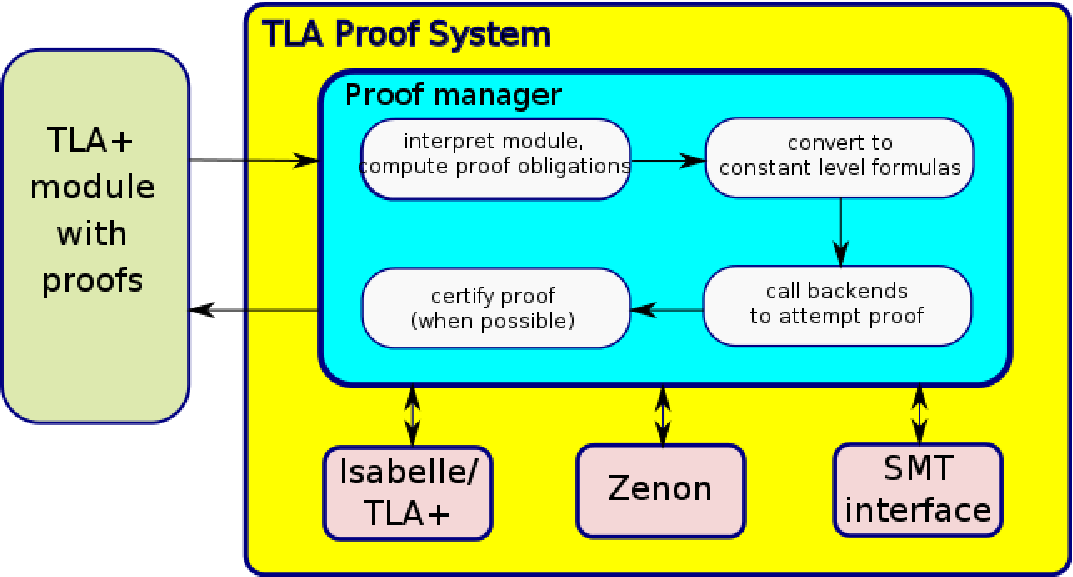
\includegraphics[width=1.0\linewidth]{architecture}}
\end{frame}

\begin{frame}
  \frametitle{Proof Manager}

  \begin{itemize}
  \item \tc{dkblue}{Interpret \tlaplus\ proof language}

    \begin{itemize}
    \o interpret module structure (imports and instantiations)
    \o manage context: known and usable facts and definitions
    \o expand operator definitions if they are usable
    \end{itemize}

  \oo \tc{dkblue}{Rewrite proof obligations to constant level}

    \begin{itemize}
    \o handle primed expressions such as\ \ \tc{dkgreen}{$Inv'$}
    \o distribute prime over (constant-level) operators
    \o introduce distinct symbols \tc{dkgreen}{$e$} and \tc{dkgreen}{$e'$}
       for atomic state expression \tc{dkgreen}{$e$}
    \end{itemize}

  \oo \tc{dkblue}{Invoke backend provers}

    \begin{itemize}
    \o user may explicitly indicate which proof method to apply
    \o optionally: certify backend proof
    \end{itemize}
  \end{itemize}
\end{frame}

%%% Local Variables: 
%%% mode: latex
%%% TeX-master: "tutorial"
%%% End: 
